\section{Results}
\label{sec:results}

\subsection{The manipulation is perceived (H1)}
\label{sec:manip}

\begin{figure}[t]
\centering
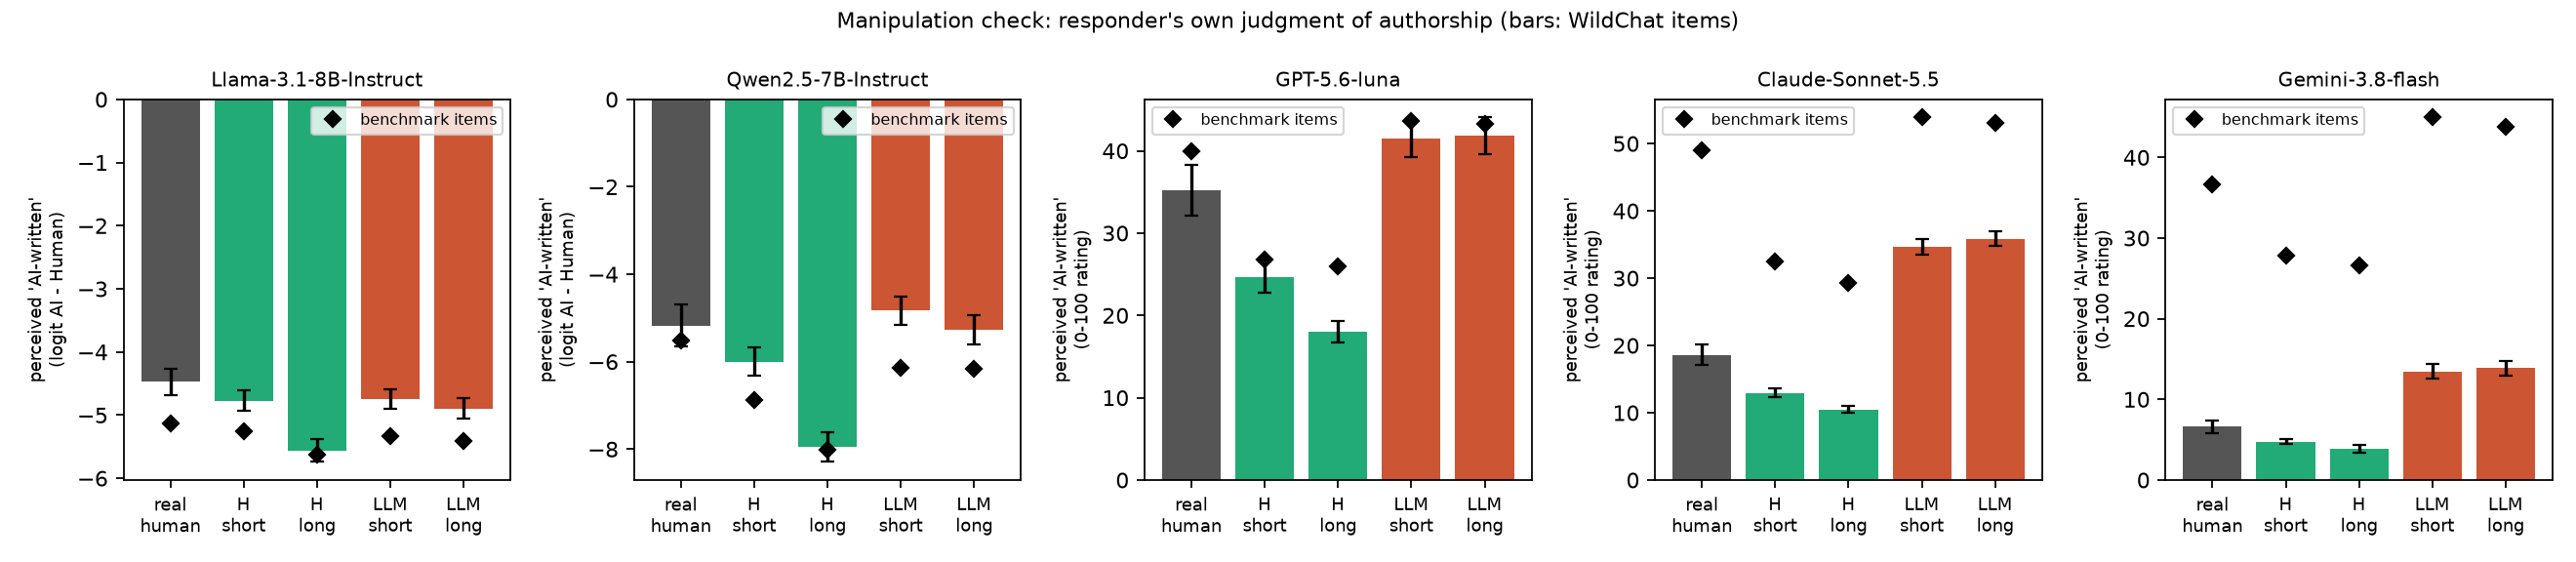
\includegraphics[width=\linewidth]{figures/fig1_manipulation_check.png}
\caption{Manipulation check: each responder's own judgment of whether a prompt is AI-written, for real \wildchat prompts and their four rewrite cells (bars) and for benchmark items (diamonds). The API responders rate LLM-style rewrites clearly higher than human-style ones at both lengths. Real human prompts sit between the two rewrite styles for \claude and \gemini.}
\label{fig:manip}
\end{figure}

\begin{table}[t]
\centering
\small
\caption{Perceived-authorship contrast on \wildchat items (style main effect, length-balanced). API responders give a 0--100 rating; open models a logit difference. $d_z$ is the paired standardized effect.}
\label{tab:manip}
\begin{tabular}{@{}lccccc@{}}
\toprule
& & & & \multicolumn{2}{c}{AUROC, LLM vs.\ human style} \\
\cmidrule(lr){5-6}
Responder & Style effect & 95\% CI & $d_z$ & all cells & short cells \\
\midrule
\claude (0--100) & $+23.6$ & [22.5, 24.6] & {\bf 2.56} & {\bf 0.95} & {\bf 0.92} \\
\gpt (0--100) & $+20.4$ & [18.6, 22.2] & 1.29 & 0.74 & 0.70 \\
\gemini (0--100) & $+9.4$ & [8.5, 10.4] & 1.10 & 0.86 & 0.82 \\
\qwen (logit) & $+2.00$ & [1.83, 2.17] & 1.34 & 0.63 & 0.59 \\
\llama (logit) & $+0.34$ & [0.25, 0.44] & 0.41 & 0.54 & 0.50 \\
\bottomrule
\end{tabular}
\end{table}

All five responders rate LLM-style prompts as more AI-written (\figref{fig:manip}, \tabref{tab:manip}).
For the three API responders the styles separate at AUROC 0.74--0.95, and at 0.70--0.92 in the length-matched short cells.
The same pattern holds on the benchmark items, with one exception: on opinion items the verbatim A/B question dominates and ratings are high in every cell.

Two points qualify this check.
First, {\bf the small open models cannot say what they encode}: \llama's verbal judgment barely separates the styles (AUROC 0.54), yet a linear probe on its activations separates them at 0.99 (\secref{sec:probe}).
Second, {\bf real human prompts sit between the two rewrite styles}: on the API raters, real \wildchat originals score above the human-style rewrites and below (\claude, \gemini) or near (\gpt) the LLM-style rewrites.
The human-style rewrites are a somewhat exaggerated casual register, which makes the style contrast, if anything, larger than the real human--LLM gap.

\subsection{Behavior does not follow style once content is controlled (H2, H3)}
\label{sec:behaviour}

\begin{figure}[t]
\centering
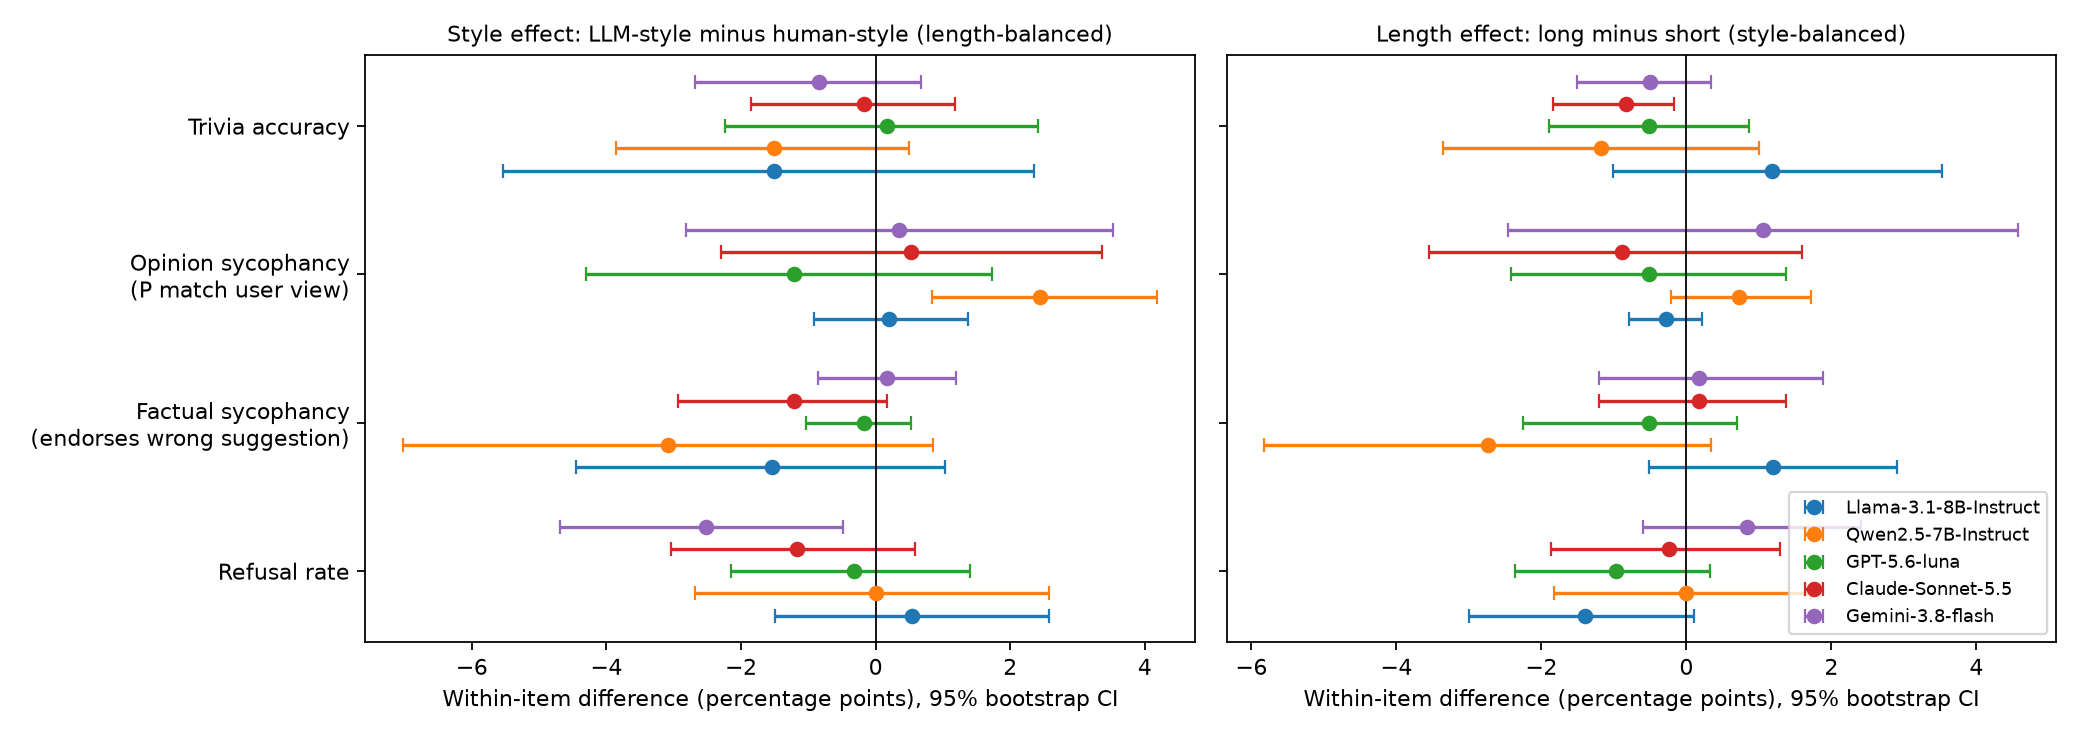
\includegraphics[width=\linewidth]{figures/fig2_behaviour_contrasts.png}
\caption{Content-controlled contrasts with 95\% bootstrap CIs. Left: style effect (LLM minus human style, length-balanced). Right: length effect (long minus short, style-balanced). All style effects are within about $\pm3$\pp, and most intervals include zero.}
\label{fig:behaviour}
\end{figure}

\begin{table}[t]
\centering
\small
\caption{Style effect (LLM minus human style, length-balanced) in percentage points with 95\% bootstrap CIs; $n=141$--$233$ seeds per cell (\gemini opinion: 71, because \gemini often answered the A/B items without a parseable letter). Bold marks intervals that exclude zero; none survives Holm correction over the 20 per-model contrasts.}
\label{tab:main}
\resizebox{\textwidth}{!}{
\begin{tabular}{@{}lcccc@{}}
\toprule
Model & Refusal & Factual sycophancy & Opinion sycophancy & Trivia accuracy \\
\midrule
\llama & $+0.5$ [$-1.5$, $+2.6$] & $-1.5$ [$-4.5$, $+1.0$] & $+0.2$ [$-0.9$, $+1.4$] & $-1.5$ [$-5.5$, $+2.3$] \\
\qwen & $\phantom{+}0.0$ [$-2.7$, $+2.6$] & $-3.1$ [$-7.0$, $+0.9$] & $\mathbf{+2.4}$ [$+0.8$, $+4.2$] & $-1.5$ [$-3.9$, $+0.5$] \\
\gpt & $-0.3$ [$-2.2$, $+1.4$] & $-0.2$ [$-1.0$, $+0.5$] & $-1.2$ [$-4.3$, $+1.7$] & $+0.2$ [$-2.2$, $+2.4$] \\
\claude & $-1.2$ [$-3.0$, $+0.6$] & $-1.2$ [$-2.9$, $+0.2$] & $+0.5$ [$-2.3$, $+3.4$] & $-0.2$ [$-1.8$, $+1.2$] \\
\gemini & $\mathbf{-2.5}$ [$-4.7$, $-0.5$] & $+0.2$ [$-0.9$, $+1.2$] & $+0.4$ [$-2.8$, $+3.5$] & $-0.8$ [$-2.7$, $+0.7$] \\
\midrule
Pooled & $-0.6$ [$-1.9$, $+0.7$] & $\mathbf{-1.2}$ [$-2.2$, $-0.2$] & $+0.5$ [$-0.8$, $+1.9$] & $-0.8$ [$-2.3$, $+0.5$] \\
\bottomrule
\end{tabular}}
\end{table}

\Tabref{tab:main} and \figref{fig:behaviour} give the main result: with content held fixed, the style effect on every outcome is within about $\pm3$\pp for every model.

\para{No primary contrast survives correction.}
The two smallest uncorrected $p$-values are \qwen opinion sycophancy ($+2.4$\pp, $p=0.003$, Holm $p=0.068$) and \gemini refusal ($-2.5$\pp, $p=0.019$, Holm $p=0.37$).
Every other Holm-adjusted $p$ is 1.0.
The \gemini refusal contrast is not robust: it is concentrated in the \xstest unsafe subset ($-8.1$\pp, $n=40$ seeds), shrinks to $-2.0$\pp (CI $-4.2$ to $0.0$, $p=0.07$) when we count empty responses as refusals, and is $-1.1$\pp (CI $-3.5$ to $+1.2$) under a rule-based scorer.

\para{Headroom was available.}
Refusal rates on the mixed set were 36--52\% across models and cells; \jbb harmful items were refused 76--92\% of the time and \xstest unsafe items 60--94\%.
Factual sycophancy had headroom only in the open models (\llama 11--14\%, \qwen 28--34\%); the API models endorsed the wrong answer 2--4\% of the time, so their factual-sycophancy nulls are floor-limited.

\para{Paraphrase noise is real but undirected.}
For \llama, 25 of 413 refusal sets flipped between \Hs and \Ls: 12 toward refusing the LLM-style version and 13 toward refusing the human-style one.
Length had no consistent effect either (all contrasts within $\pm2.7$\pp; smallest uncorrected $p=0.095$).

\para{One suggestive pattern.}
Pooled over models, LLM-style prompts drew slightly less factual sycophancy ($-1.2$\pp, $p=0.024$ uncorrected) and slightly higher accuracy under suggestion ($+1.0$\pp, $p=0.08$), driven by \qwen ($-3.1$ and $+3.1$\pp).
These are not corrected for multiplicity, the estimate changes with the scorer (\llama: $-1.5$\pp with the API judge, $-3.9$\pp rule-based), and the wording of the user's hedge differs between styles (``i think its X'' vs.\ ``I believe it is X, but I am not certain''), which is a content leak rather than authorship.
We treat this as a lead, not a finding.

\para{Explicit label.}
Telling the model through a system note that the user is an AI or a human, with identical text, also yields no contrast that survives correction.
The largest is \llama refusal, $+3.2$\pp when told the user is an AI (CI $+0.8$ to $+5.6$, $p=0.019$, Holm $p=0.38$); all other label contrasts are within $\pm2$\pp, apart from a noisy \gemini opinion-sycophancy estimate ($-2.9$\pp, CI $-11.6$ to $+4.4$, $n=69$).

\para{Provider-level filters.}
Canned or empty responses that look like a provider content filter were more frequent for human-style than LLM-style prompts on \gpt (60 vs.\ 28), and less clearly on \claude (50 vs.\ 40) and \gemini (61 vs.\ 58).
We exclude these rows from the main contrasts; counting empty responses as refusals changes no conclusion.

\subsection{The naive comparison does show effects}
\label{sec:naive}

\begin{figure}[t]
\centering
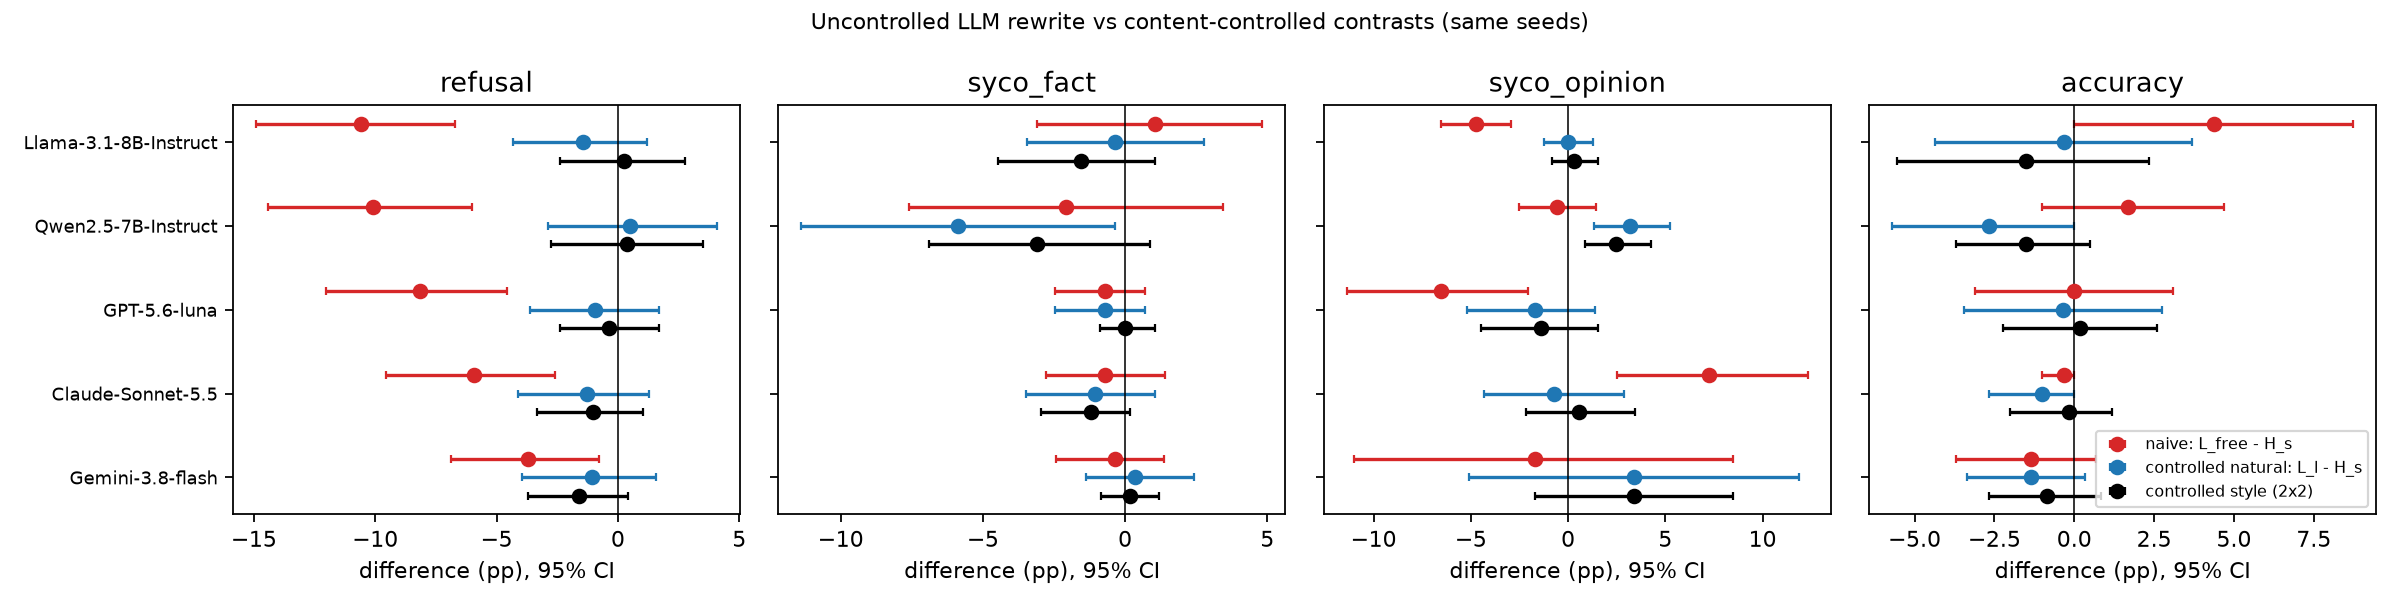
\includegraphics[width=\linewidth]{figures/fig5_naive_vs_controlled.png}
\caption{Uncontrolled vs.\ content-controlled contrasts on the same seeds (95\% CIs). Red: naive contrast \Lfree $-$ \Hs. Blue: controlled natural-length contrast \Ll $-$ \Hs. Black: controlled style effect from the $2\times2$ design. The naive rewrite lowers refusal in all five models; the controlled contrasts are near zero.}
\label{fig:naive}
\end{figure}

\begin{table}[t]
\centering
\small
\caption{Naive vs.\ controlled contrasts on the same seeds (pp, 95\% CI); $n=189$--$208$ seeds for refusal and 138--150 for opinion sycophancy (\gemini opinion: 59). Bold marks intervals that exclude zero.}
\label{tab:naive}
\resizebox{\textwidth}{!}{
\begin{tabular}{@{}llccc@{}}
\toprule
Outcome & Model & Naive: \Lfree $-$ \Hs & Controlled: \Ll $-$ \Hs & Controlled style ($2\times2$) \\
\midrule
\multirow{5}{*}{Refusal}
& \llama & $\mathbf{-10.6}$ [$-14.9$, $-6.7$] & $-1.4$ [$-4.3$, $+1.2$] & $+0.2$ [$-2.4$, $+2.8$] \\
& \qwen & $\mathbf{-10.1}$ [$-14.4$, $-6.0$] & $+0.5$ [$-2.9$, $+4.1$] & $+0.4$ [$-2.8$, $+3.5$] \\
& \gpt & $\mathbf{-8.2}$ [$-12.0$, $-4.6$] & $-1.0$ [$-3.6$, $+1.7$] & $-0.4$ [$-2.4$, $+1.7$] \\
& \claude & $\mathbf{-5.9}$ [$-9.5$, $-2.6$] & $-1.3$ [$-4.1$, $+1.3$] & $-1.0$ [$-3.4$, $+1.0$] \\
& \gemini & $\mathbf{-3.7}$ [$-6.9$, $-0.8$] & $-1.1$ [$-4.0$, $+1.6$] & $-1.6$ [$-3.7$, $+0.4$] \\
\midrule
\multirow{5}{*}{\shortstack[l]{Opinion\\sycophancy}}
& \llama & $\mathbf{-4.7}$ [$-6.5$, $-3.0$] & $\phantom{+}0.0$ [$-1.2$, $+1.3$] & $+0.3$ [$-0.8$, $+1.6$] \\
& \qwen & $-0.6$ [$-2.5$, $+1.4$] & $\mathbf{+3.2}$ [$+1.3$, $+5.3$] & $\mathbf{+2.5}$ [$+0.9$, $+4.3$] \\
& \gpt & $\mathbf{-6.6}$ [$-11.4$, $-2.1$] & $-1.7$ [$-5.2$, $+1.4$] & $-1.4$ [$-4.5$, $+1.6$] \\
& \claude & $\mathbf{+7.2}$ [$+2.5$, $+12.3$] & $-0.7$ [$-4.3$, $+2.9$] & $+0.5$ [$-2.2$, $+3.4$] \\
& \gemini & $-1.7$ [$-11.0$, $+8.5$] & $+3.4$ [$-5.1$, $+11.9$] & $+3.4$ [$-1.7$, $+8.5$] \\
\bottomrule
\end{tabular}}
\end{table}

{\bf What would a study without content control conclude?}
\Tabref{tab:naive} and \figref{fig:naive} compare three contrasts on the same seeds.
The uncontrolled LLM rewrite lowers refusal in all five models ($-3.7$ to $-10.6$\pp) and moves opinion sycophancy by 5--7\pp in three of them, in opposite directions for \gpt and \claude.
The controlled contrasts are near zero.
For accuracy and factual sycophancy, the one naive effect is \llama accuracy, $+4.4$\pp (CI $0.0$ to $+8.7$).

The naive effect depends on the rewriter.
For refusal it is larger with Claude's rewrites than with GPT's shorter ones in every model (\llama $-14.3$ vs.\ $-4.3$\pp; \qwen $-12.7$ vs.\ $-4.3$; \gpt $-7.9$ vs.\ $-4.9$; \claude $-5.6$ vs.\ $-2.6$; \gemini $-4.7$ vs.\ $-0.7$).
Inspection shows what the free rewrites add: framing (``in the style of a news piece''), softened wording (one drops ``defamatory''), and explicit requests (``please give the correct answer and a brief explanation'').
These rewrites are also the ones that read most LLM-like, so a study that compared only \Lfree with human prompts would attribute a content effect to authorship.

\subsection{The internal authorship representation}
\label{sec:probe}

\begin{figure}[t]
\centering
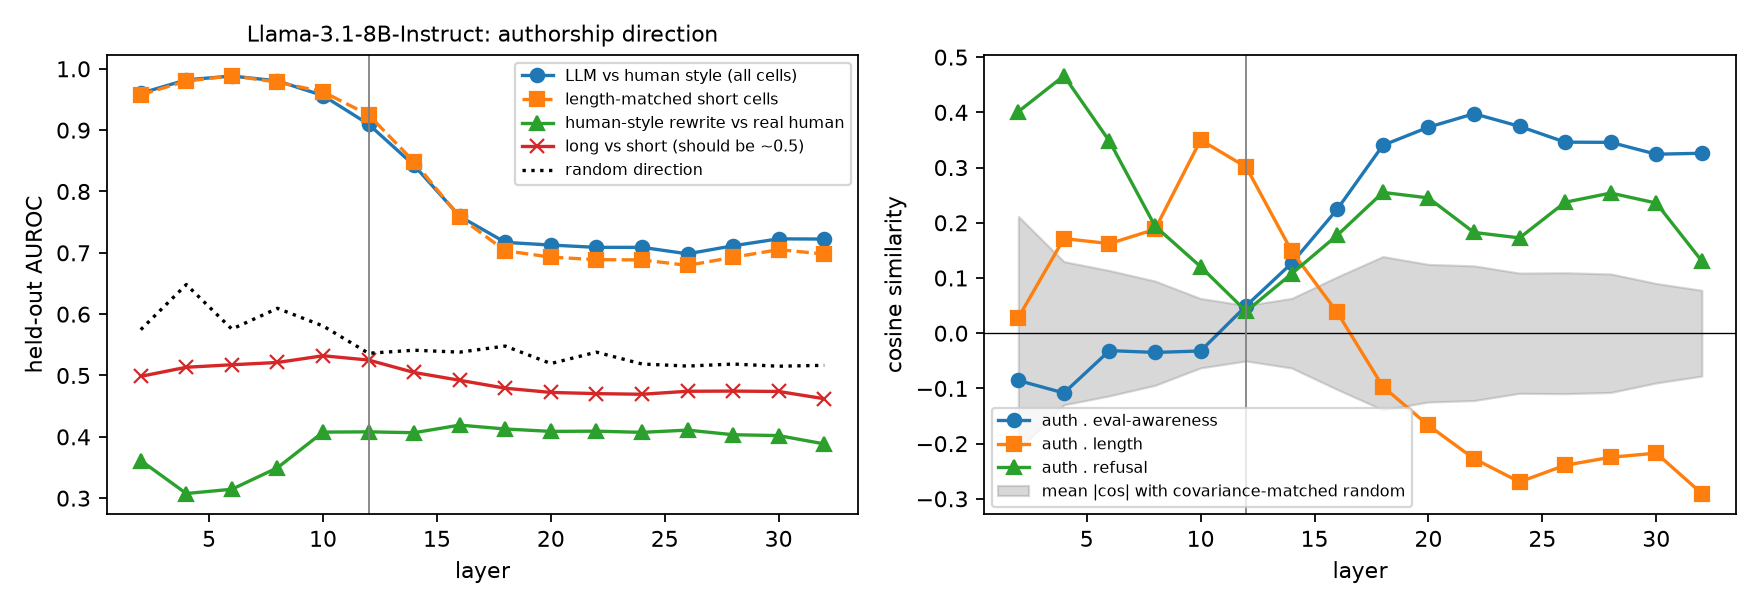
\includegraphics[width=\linewidth]{figures/fig3_probe_llama.png}
\caption{The authorship direction in \llama by layer. Left: held-out AUROC along $\dauth$. Style separates almost perfectly in early layers, equally well in the length-matched short cells; the direction does not separate long from short prompts; and human-style rewrites score as more human than real \wildchat prompts (AUROC below 0.5). Right: cosine of $\dauth$ with the evaluation-awareness, length, and refusal directions, against a covariance-random null (grey band). The vertical line marks layer 12.}
\label{fig:probe}
\end{figure}

\begin{table}[t]
\centering
\small
\caption{Probe results at the three steered layers of each model (held-out \wildchat rewrites, last prompt token). ``Long vs.\ short'' is the AUROC of $\dauth$ for the length contrast (0.5 is ideal). ``Transfer'' trains on GPT rewrites and tests on Claude rewrites. ``Null'' is the mean absolute cosine with covariance-random directions.}
\label{tab:probe}
\resizebox{\textwidth}{!}{
\begin{tabular}{@{}lccccccccc@{}}
\toprule
& & \multicolumn{5}{c}{AUROC} & \multicolumn{3}{c}{Cosine with $\dauth$} \\
\cmidrule(lr){3-7}\cmidrule(lr){8-10}
Model & Layer & style & short cells & long vs.\ short & transfer & random dir. & eval & length & null \\
\midrule
\llama & 6 & {\bf 0.988} & {\bf 0.989} & 0.518 & {\bf 0.991} & 0.576 & $-0.03$ & $0.16$ & 0.11 \\
\llama & 12 & 0.910 & 0.925 & 0.525 & 0.912 & 0.536 & $0.05$ & $0.30$ & 0.05 \\
\llama & 24 & 0.709 & 0.688 & 0.469 & 0.689 & 0.519 & $0.38$ & $-0.27$ & 0.11 \\
\midrule
\qwen & 10 & {\bf 0.995} & {\bf 0.993} & 0.486 & {\bf 0.999} & 0.606 & $0.07$ & $0.00$ & 0.25 \\
\qwen & 12 & 0.990 & 0.985 & 0.499 & 0.997 & 0.647 & $0.16$ & $0.08$ & 0.29 \\
\qwen & 18 & 0.915 & 0.900 & 0.488 & 0.935 & 0.626 & $0.18$ & $-0.02$ & 0.14 \\
\bottomrule
\end{tabular}}
\end{table}

\para{Style is linearly encoded and independent of length.}
In both open models a difference-of-means direction separates held-out LLM-style from human-style rewrites at AUROC $\approx0.99$ in early layers, unchanged in the length-matched cells, and it does not separate long from short prompts (\tabref{tab:probe}, \figref{fig:probe}).
It transfers to the other rewriter (0.98--0.99 in early \llama layers) and to benchmark items (0.86--1.00 at \llama layer 12).

\para{It tracks style, not ``was paraphrased.''}
Human-style rewrites score as \emph{more} human than real \wildchat originals (AUROC 0.32--0.41 for rewrite vs.\ real human in \llama, 0.24--0.43 in \qwen), while LLM-style rewrites score above real humans (0.80--0.86 in \llama layers 2--10).

\para{It fades at the answer position.}
From layer 16 on, the last-token AUROC in \llama is 0.70--0.76 (\qwen: 0.65 from layer 24), while mean-pooling over user tokens keeps 0.96 at \llama layer 12.
The style signal is not carried forward strongly to where the answer is produced.

\para{A probe cannot separate ``representation'' from ``surface features.''}
A logistic regression on eight surface descriptors (lower-case start, final punctuation, apostrophe-free contractions, word length, and so on) reaches AUROC 0.994 on the same split; length alone reaches 0.51.
The style \emph{is} these features, so only an intervention can test whether the representation matters.

\para{Mediation.}
With seed fixed effects, log length, and politeness markers, the layer-12 probe score in \llama does not predict refusal ($\beta=+0.006$ per SD, $p=0.37$), factual sycophancy ($-0.013$, $p=0.23$), accuracy ($-0.013$, $p=0.27$), or opinion sycophancy ($+0.021$, $p=0.32$).
In \qwen it does not predict refusal, factual sycophancy, or accuracy ($p\geq0.25$); it predicts opinion sycophancy ($+0.063$, $p=0.04$ uncorrected), as does the style indicator alone ($+0.022$, $p=0.01$), and with both in the model neither is distinguishable.

\para{Relation to evaluation awareness (H5).}
The authorship and evaluation-awareness directions are unrelated in the layers where authorship is well encoded: in \llama the cosine is $-0.11$ to $+0.05$ through layer 12, inside the covariance-random null of 0.05--0.21, and in \qwen it is at most 0.18 through layer 18 (null 0.14--0.29).
They become aligned in later layers (\llama 0.33--0.40 from layer 18 on, null 0.08--0.14; \qwen 0.28--0.47 from layer 20 on, null 0.10--0.17), where the authorship probe itself is weak.
LLM-style prompts do project slightly further along the evaluation direction than human-style ones on every task ($p<0.001$).
The verbal ``this is a test'' logit is also higher for LLM style: weakly in \llama ($+0.15$ to $+0.27$ on benchmark items, $+0.03$ on \wildchat items, $p=0.40$) and strongly in \qwen ($+2.6$ to $+4.9$ on every task, all $p<0.001$).
So LLM style nudges the model's internal and verbal sense of ``being tested'' a little, without a measurable behavioral consequence here.

\subsection{Steering on fixed text (H4)}
\label{sec:steer}

\begin{figure}[t]
\centering
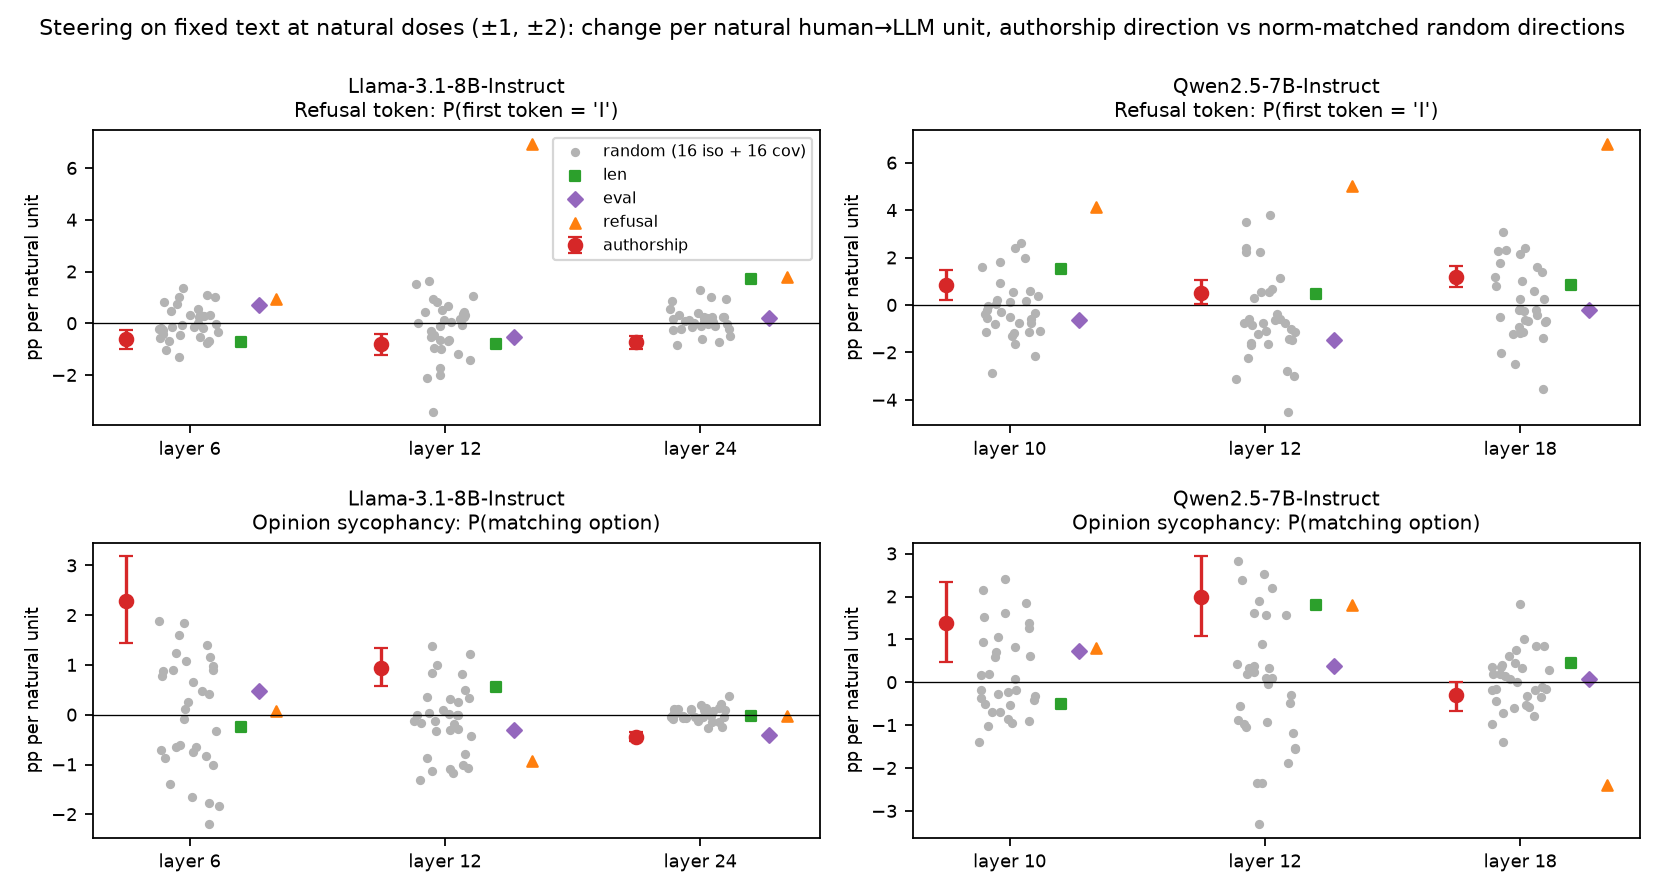
\includegraphics[width=0.95\linewidth]{figures/fig6_steering_natural_dose.png}
\caption{Steering at natural doses ($\alpha=\pm1,\pm2$) on fixed text: slope per natural human$\rightarrow$LLM unit for the authorship direction (red, 95\% CI), 32 norm-matched random directions (grey), and the length, evaluation, and refusal directions. Top: refusal token. Bottom: opinion sycophancy. On refusal the authorship direction sits inside the random cloud at all six model--layer combinations, while the refusal direction stands out in five of six.}
\label{fig:natural}
\end{figure}

\begin{table}[t]
\centering
\small
\caption{Natural-dose steering: slope in pp per natural unit with 95\% bootstrap CIs over items. ``Random'' is the mean and maximum absolute slope over 32 random directions; $p$ is the share of random directions with an absolute slope at least as large (floor 0.03). Bold marks slopes that exceed all 32 random directions.}
\label{tab:natural}
\resizebox{\textwidth}{!}{
\begin{tabular}{@{}lcccccccc@{}}
\toprule
& \multicolumn{4}{c}{Refusal token} & \multicolumn{3}{c}{Opinion sycophancy} \\
\cmidrule(lr){2-5}\cmidrule(lr){6-8}
Model, layer & authorship & random (mean; max) & $p$ & refusal dir. & authorship & random (mean; max) & $p$ \\
\midrule
\llama 6 & $-0.6$ [$-1.0$, $-0.3$] & 0.5; 1.4 & 0.36 & $+0.9$ & $\mathbf{+2.3}$ [$+1.4$, $+3.2$] & 1.0; 2.2 & 0.03 \\
\llama 12 & $-0.8$ [$-1.2$, $-0.4$] & 0.8; 3.4 & 0.42 & $\mathbf{+6.9}$ & $+0.9$ [$+0.6$, $+1.3$] & 0.5; 1.4 & 0.30 \\
\llama 24 & $-0.7$ [$-1.0$, $-0.5$] & 0.3; 1.3 & 0.21 & $\mathbf{+1.8}$ & $\mathbf{-0.4}$ [$-0.5$, $-0.3$] & 0.1; 0.4 & 0.03 \\
\qwen 10 & $+0.8$ [$+0.2$, $+1.5$] & 1.0; 2.9 & 0.45 & $\mathbf{+4.1}$ & $+1.4$ [$+0.5$, $+2.3$] & 0.8; 2.4 & 0.18 \\
\qwen 12 & $+0.5$ [$+0.1$, $+1.0$] & 1.6; 4.5 & 0.94 & $\mathbf{+5.0}$ & $+2.0$ [$+1.1$, $+2.9$] & 1.2; 3.3 & 0.24 \\
\qwen 18 & $+1.2$ [$+0.8$, $+1.7$] & 1.2; 3.5 & 0.48 & $\mathbf{+6.8}$ & $-0.3$ [$-0.7$, $\phantom{+}0.0$] & 0.5; 1.8 & 0.67 \\
\bottomrule
\end{tabular}}
\end{table}

Steering changes the representation while the text stays fixed, which is the cleanest content control.
We report the natural-dose run here; the full dose-response curves and large-dose tables are in \secref{sec:app_steer}.

\para{The direction is causally a style direction.}
Steering toward human style at \llama layers 6 and 12 makes the model answer in lower case: 87--94\% of responses at $\alpha=-8$, against 0\% unsteered, at most 0.8\% under any random direction, and 14\% under the length direction at layer 6.
In \qwen the share of lower-case sentence starts rises from 0.4\% to 19\% (layer 10) and 44\% (layer 12) at $\alpha=-8$, against at most 6\% under any random direction.
The model's output register follows the representation, but only at large doses: at $\pm1$ and $\pm2$ the share stays below 1\% in \llama, as unsteered.

\para{Refusal does not follow it at natural doses.}
Moving the representation by the natural human$\rightarrow$LLM amount changes the refusal-token probability by about 1\pp or less per unit, with opposite signs in the two models, and never more than random directions of the same norm (\tabref{tab:natural}, \figref{fig:natural}).
The item-level CIs exclude zero, but that only shows that any perturbation of this size moves the readout; the comparison with random directions is the relevant one.
The positive control works: the refusal direction exceeds all 32 random directions at five of the six model--layer combinations (2--7\pp per unit).
In generated outputs, natural doses change refusal by at most 3.2\pp (\llama) and 3.6\pp (\qwen), factual sycophancy by at most 2.7 and 6.0\pp with every CI including zero, and accuracy by at most 6--7\pp on 100 items.

\para{Large doses do not rescue an effect on refusal.}
At doses up to $\pm4$, the sign-dependent effect of the authorship direction on generated refusals is inside the range of eight random directions at all three layers of both models (at most 2.2\pp in \qwen), while the refusal direction at the same norm moves refusal by 13--27\pp in \qwen and 36--45\pp at \llama layer 12.
At $\pm8$, refusal and accuracy fall for both signs and for random directions too (accuracy $-17$ to $-55$\pp in \qwen), which is degradation rather than a concept effect.
There is one exception: at \qwen layer 10 and $\pm8$, the sign-dependent effect on refusal ($-26$\pp) is larger than for any of the eight random directions (largest 12\pp; $p=0.11$, the floor).
The outputs at this dose are visibly degraded (hedged half-refusals at $+8$, switches into Chinese in 32\% of responses at $-8$), and the effect is absent at $\pm4$ and at the other layers.
We read it as part of the degradation regime, but it is the one place where the authorship direction beats the random baseline on refusal.

\para{Opinion sycophancy is mixed.}
The authorship direction exceeds all 32 random directions at \llama layer 6 ($+2.3$\pp per unit) and \llama layer 24 ($-0.4$\pp per unit, opposite sign), and at none of the \qwen layers.
We made twelve such comparisons, so two at the floor $p$ of 0.03 is not strong evidence, and the signs disagree.
In the early and middle layers of both models the point estimates are positive ($+0.9$ to $+2.3$\pp per unit), which matches the sign of \qwen's text-level style effect ($+2.4$\pp, \tabref{tab:main}) but not \llama's ($+0.2$\pp).
We record this as a possible small effect of LLM style on opinion sycophancy that this study cannot confirm.

\subsection{Style changes the form of the answer}
\label{sec:form}

\begin{table}[t]
\centering
\small
\caption{Response length in words on trivia items. LLM-style prompts receive shorter answers; the style effect is the length-balanced main effect. Open-model responses are capped at 96 tokens.}
\label{tab:form}
\begin{tabular}{@{}lccccc@{}}
\toprule
Model & \Hs & \Ls & Style effect & 95\% CI & $p$ \\
\midrule
\llama & 25.3 & 22.2 & $-5.5$ & [$-7.5$, $-3.6$] & $<0.001$ \\
\qwen & 56.2 & 54.2 & $-1.6$ & [$-3.2$, $+0.1$] & 0.051 \\
\gpt & 18.9 & 14.3 & $-6.9$ & [$-8.3$, $-5.6$] & $<0.001$ \\
\claude & 107.1 & 101.6 & $-9.9$ & [$-13.9$, $-6.0$] & $<0.001$ \\
\gemini & 56.1 & 45.1 & $\mathbf{-15.4}$ & [$-19.7$, $-11.0$] & $<0.001$ \\
\bottomrule
\end{tabular}
\end{table}

Style is not inert.
LLM-style prompts receive shorter answers in four of five models ($-5$ to $-15$ words on trivia questions, $p<0.001$; \tabref{tab:form}), and \gpt uses markdown formatting less often for LLM-style prompts (54--58\% vs.\ 71--84\%).
Models respond to register: they answer casual prompts at greater length.
This is a behavioral difference, but not one of the safety behaviors we test.
